\documentclass[11pt]{article}
\usepackage[english]{babel}
% Shared preamble for report_en.tex and report_tr.tex
\usepackage[T1]{fontenc}
\usepackage[utf8]{inputenc}
\usepackage{lmodern}
\usepackage{microtype}
\usepackage[a4paper,margin=2.4cm]{geometry}
\usepackage{amsmath,amssymb}
\usepackage{graphicx}
\usepackage{booktabs}
\usepackage{tabularx}
\usepackage{multirow}
\usepackage{xcolor}
\usepackage{float}
\usepackage{caption}
\usepackage{subcaption}
\usepackage{enumitem}
\usepackage{listings}
\usepackage{tikz}
\usetikzlibrary{arrows.meta,positioning,shapes.geometric,fit,calc}
\usepackage{fancyhdr}
\usepackage[hidelinks]{hyperref}

\graphicspath{{../reports/figures/}}
\setlength{\parskip}{0.45em}
\setlength{\parindent}{0pt}
\captionsetup{font=small,labelfont=bf}
\setlist{itemsep=0.15em,topsep=0.3em}

\definecolor{ink}{HTML}{0B0B0B}
\definecolor{ink2}{HTML}{52514E}
\definecolor{accent}{HTML}{2A78D6}
\definecolor{alarm}{HTML}{E34948}
\definecolor{codebg}{HTML}{F6F6F4}
\definecolor{codekw}{HTML}{4A3AA7}
\definecolor{codestr}{HTML}{0F7B55}
\definecolor{codecom}{HTML}{8A8984}

\lstdefinestyle{py}{
  language=Python,
  basicstyle=\ttfamily\footnotesize,
  keywordstyle=\color{codekw}\bfseries,
  stringstyle=\color{codestr},
  commentstyle=\color{codecom}\itshape,
  backgroundcolor=\color{codebg},
  frame=single,
  rulecolor=\color{codebg},
  framesep=4pt,
  numbers=left,
  numberstyle=\tiny\color{codecom},
  numbersep=6pt,
  showstringspaces=false,
  breaklines=true,
  breakatwhitespace=true,
  columns=fullflexible,
  keepspaces=true,
  tabsize=4,
  upquote=true,
  morekeywords={self,None,True,False},
  literate={×}{{$\times$}}1 {≈}{{$\approx$}}1 {→}{{$\to$}}1
}
\lstdefinestyle{plain}{
  basicstyle=\ttfamily\footnotesize,
  backgroundcolor=\color{codebg},
  frame=single,
  rulecolor=\color{codebg},
  framesep=4pt,
  columns=fullflexible,
  keepspaces=true,
  breaklines=true,
  upquote=true
}
\lstset{style=py}

\pagestyle{fancy}
\fancyhf{}
\renewcommand{\headrulewidth}{0.3pt}
\fancyfoot[C]{\thepage}

\newcommand{\code}[1]{\texttt{#1}}
\newcommand{\figw}{\textwidth}

% Pipeline diagram (language-neutral labels are passed as arguments)
\newcommand{\pipeline}[6]{%
\begin{tikzpicture}[
  node distance=0.55cm,
  box/.style={draw=accent!70,fill=accent!6,rounded corners=3pt,align=center,
              minimum height=1.25cm,text width=2.35cm,font=\small},
  arr/.style={-{Stealth[length=2.4mm]},thick,draw=ink2}]
  \node[box] (a) {#1};
  \node[box,right=of a] (b) {#2};
  \node[box,right=of b] (c) {#3};
  \node[box,right=of c] (d) {#4};
  \node[box,right=of d,draw=alarm!80,fill=alarm!6] (e) {#5};
  \draw[arr] (a) -- (b); \draw[arr] (b) -- (c); \draw[arr] (c) -- (d); \draw[arr] (d) -- (e);
  \node[below=0.25cm of c,font=\footnotesize\color{ink2},text width=12cm,align=center] {#6};
\end{tikzpicture}}

\fancyhead[L]{\small\color{ink2}Bearing Early Fault Warning}
\fancyhead[R]{\small\color{ink2}Technical Report}

\title{\textbf{Bearing Early Fault Warning}\\[0.3em]
\large Unsupervised anomaly detection and early-warning on the NASA/IMS run-to-failure bearing dataset\\[0.2em]
\normalsize Technical Report}
\author{Ecem Aydemir}
\date{October 2026}

\begin{document}
\maketitle
\thispagestyle{empty}

\begin{abstract}
\noindent
Rolling-element bearings are among the most common causes of failure in rotating machinery, and
failure labels are almost never available in practice. This report describes a complete,
reproducible early-warning system that learns what \emph{healthy} vibration looks like from the first
part of a machine's life and raises a debounced alarm when a bearing drifts away from it. The system
reduces each one-second, 20\,kHz vibration snapshot to 18 physically meaningful condition indicators
(time-domain statistics, band energies and envelope-spectrum energy at the bearing defect
frequencies), compares four detectors (an RMS threshold baseline, Mahalanobis distance, Isolation
Forest and an LSTM autoencoder) and adds an envelope-spectrum diagnosis of the likely defect. On the
development test (IMS test~2) every detector raises a persistent alarm on the failing bearing about
\textbf{74 hours (45\,\% of the run) before the end of the test} and correctly identifies an
\textbf{outer-race} defect. On the two held-out tests the results expose a clear trade-off between lead
time and false alarms, and an honest limitation: operating-condition changes after machine stops
look like anomalies. The work is delivered as an open-source Python package with a one-command
pipeline, unit tests, a walkthrough notebook and an interactive Streamlit dashboard.
\end{abstract}

\tableofcontents
\newpage

%=====================================================================
\section{Introduction}
%=====================================================================

\subsection{Problem}
Predictive maintenance aims to repair a machine \emph{shortly before} it fails: late enough to use most
of a component's life, early enough to plan the intervention. For rotating machines, vibration is the
richest source of information, and bearings are the component that fails most often. A
sensor-equipped machine streams vibration data continuously, but almost never comes with labels
saying ``this bearing is now degrading''. Failures are rare, expensive and different from each other,
so a model trained to classify known failures will not be available for a new machine.

The question this project answers is therefore:
\begin{quote}
\emph{Using only data from a period in which the machine is assumed healthy, can we warn an operator
early, reliably and with few false alarms that a bearing is starting to fail, and say what kind of
defect it probably is?}
\end{quote}

\subsection{Approach in one paragraph}
Every vibration snapshot is turned into a compact vector of condition indicators. The first 25\,\% of
each run is treated as healthy and used to fit an anomaly detector; the next 10\,\% sets an alarm
threshold. From then on the detector scores every new snapshot, an alarm is raised when 4 of the last
6 scores exceed the threshold, and the defect frequency whose envelope energy has grown most names the
likely failure mode. The system is evaluated on three run-to-failure experiments by the number of
hours between the alarm and the end of the test (\emph{lead time}) and by the number of alarms raised
while the machine was still healthy (\emph{false alarms}).

\subsection{Contributions}
\begin{itemize}
  \item A leakage-free, time-ordered evaluation protocol for the IMS dataset, applied to all three
        tests and all failed bearings, with test~2 used for development and tests~1 and~3 held out.
  \item Physically grounded features including envelope analysis at the bearing defect frequencies,
        computed for the exact bearing geometry of the test rig.
  \item A comparison of a classic baseline, two classical machine-learning detectors and a
        deep-learning sequence model under identical splits, thresholds and alarm logic.
  \item Operator-facing alarm logic (debouncing, persistence, first-to-alarm localisation and defect
        diagnosis) and an interactive dashboard that replays a test as a live stream.
  \item A reproducible software package: configuration file, Makefile, unit tests, committed feature
        tables (3\,MB) so that every result can be regenerated without downloading 6\,GB of raw data.
\end{itemize}

\subsection{Relation to an earlier attempt}
This project restarts an earlier notebook (2025) that trained an LSTM autoencoder on the same dataset.
Reviewing it revealed several methodological problems that invalidate its results. They are worth
listing because they are common with this dataset and motivated the design decisions in
Section~\ref{sec:design}:
\begin{enumerate}
  \item \textbf{The model was trained on failure data.} The training set was the \emph{last} million
        samples of the run, i.e.\ the period in which the bearing was failing, and the same data was
        then used for testing.
  \item \textbf{The wrong bearing was monitored.} Only the first channel of test~1 (bearing~1) was
        used, but in test~1 bearings~3 and~4 fail and bearing~1 survives.
  \item \textbf{Time was lost.} All 2\,156 files were concatenated into one signal and cut into windows
        of 50 samples (2.5\,ms). Without a time axis the question ``how many hours before failure did
        it warn?'' cannot be answered.
  \item \textbf{Leakage between training and validation.} Overlapping windows were shuffled before the
        train/validation split, so the validation loss was optimistic.
\end{enumerate}
The idea of the earlier work (learn ``normal'' with an autoencoder and use reconstruction error as an
anomaly score) is kept; it is the LSTM autoencoder detector in this report, now set up correctly.

%=====================================================================
\section{Background}
%=====================================================================

\subsection{Rolling-element bearings and their defects}
A rolling-element bearing consists of an inner race (mounted on the shaft), an outer race (mounted in
the housing), rolling elements (balls or rollers) and a cage that keeps the rolling elements apart.
Fatigue, contamination or poor lubrication create a local defect (a spall or crack) on one of these
surfaces. Every time a rolling element passes over the defect it produces a short mechanical impact.
These impacts repeat at a rate that depends only on the bearing geometry and the shaft speed, and they
excite the structural resonances of the bearing and housing, typically in the kHz range.

For a shaft frequency $f_r$, $n$ rolling elements of diameter $d$, pitch diameter $D$ and contact angle
$\phi$, the characteristic defect frequencies are
\begin{align}
\text{BPFO} &= \frac{n}{2} f_r \left(1 - \frac{d}{D}\cos\phi\right) && \text{(ball pass frequency, outer race)}\\
\text{BPFI} &= \frac{n}{2} f_r \left(1 + \frac{d}{D}\cos\phi\right) && \text{(ball pass frequency, inner race)}\\
\text{BSF}  &= \frac{D}{2d} f_r \left(1 - \left(\frac{d}{D}\cos\phi\right)^2\right) && \text{(ball spin frequency, rolling element)}\\
\text{FTF}  &= \frac{f_r}{2} \left(1 - \frac{d}{D}\cos\phi\right) && \text{(fundamental train / cage frequency)}
\end{align}

The IMS test rig uses Rexnord ZA-2115 double-row bearings with $n=16$ rollers per row,
$d = 0.331$\,in, $D = 2.815$\,in and $\phi = 15.17^\circ$ at 2000\,rpm ($f_r = 33.3$\,Hz).
Table~\ref{tab:freqs} lists the resulting frequencies; the implementation is shown in
Listing~\ref{lst:freqs}.

\begin{table}[H]
\centering
\caption{Characteristic defect frequencies of the ZA-2115 bearing at 2000\,rpm.}
\label{tab:freqs}
\begin{tabular}{lrl}
\toprule
Frequency & Value [Hz] & Defect it indicates \\
\midrule
BPFO & 236.4 & outer race \\
BPFI & 296.9 & inner race \\
BSF  & 139.9 & rolling element \\
FTF  & 14.8  & cage \\
\bottomrule
\end{tabular}
\end{table}

\begin{lstlisting}[caption={Defect frequencies from the bearing geometry (\code{src/bearing\_efw/dataset.py}).},label=lst:freqs]
FS = 20_480  # sampling rate [Hz]
SHAFT_HZ = 2000 / 60.0
N_ROLLERS, ROLLER_D, PITCH_D, CONTACT_ANGLE_DEG = 16, 0.331, 2.815, 15.17

def fault_frequencies(fr: float = SHAFT_HZ) -> dict[str, float]:
    """Characteristic defect frequencies [Hz] for the ZA-2115 bearing."""
    ratio = ROLLER_D / PITCH_D * np.cos(np.deg2rad(CONTACT_ANGLE_DEG))
    return {
        "bpfo": N_ROLLERS / 2 * fr * (1 - ratio),  # outer race
        "bpfi": N_ROLLERS / 2 * fr * (1 + ratio),  # inner race
        "bsf": PITCH_D / (2 * ROLLER_D) * fr * (1 - ratio**2),  # rolling element
        "ftf": fr / 2 * (1 - ratio),  # cage
    }
\end{lstlisting}

\subsection{Vibration condition indicators}
\paragraph{Time-domain statistics.} For a zero-mean snapshot $x_1,\dots,x_N$:
\begin{align}
\text{RMS} &= \sqrt{\tfrac{1}{N}\textstyle\sum_i x_i^2}, &
\text{kurtosis} &= \frac{\tfrac{1}{N}\sum_i x_i^4}{\text{RMS}^4}, &
\text{crest factor} &= \frac{\max_i |x_i|}{\text{RMS}}.
\end{align}
RMS measures overall vibration energy and is the indicator used by most industrial standards (e.g.\
ISO 10816/20816). Kurtosis equals 3 for Gaussian noise and grows when the signal contains sharp
impacts, which makes it sensitive to early, localized defects even before the energy rises.
Crest, shape ($\text{RMS}/\overline{|x|}$) and impulse ($\max|x|/\overline{|x|}$) factors are related
impulsiveness measures; skewness captures asymmetry.

\paragraph{Spectral band energies.} The fraction of the power spectrum in six bands
(0--1, 1--2, 2--4, 4--6, 6--8 and 8--10.24\,kHz) and the spectral centroid describe \emph{where} the
energy sits. A developing defect shifts energy towards the high-frequency resonances.

\paragraph{Envelope analysis.} Defect impacts are short and excite high-frequency resonances; their
\emph{repetition rate} (e.g.\ BPFO) is invisible in the raw spectrum because it is hidden under the
resonance. Envelope analysis recovers it in three steps \cite{randall2011}:
\begin{enumerate}
  \item band-pass filter the signal around the resonance region (here 2--8\,kHz, 4th-order
        Butterworth, zero-phase),
  \item take the magnitude of the analytic signal (Hilbert transform), which is the envelope of the
        amplitude-modulated resonance,
  \item compute the spectrum of the envelope; a localized defect produces a peak at its
        characteristic frequency and its harmonics.
\end{enumerate}
The feature used here is the share of envelope-spectrum energy (5--1000\,Hz) that lies within
$\pm3$\,Hz of the first three harmonics of BPFO, BPFI and BSF.

\subsection{Unsupervised anomaly detection}
Because no failure labels are used, all detectors are \emph{one-class} or \emph{novelty} detectors:
they are fitted on healthy data only and assign a score that grows as a new observation becomes less
similar to it.

\paragraph{Mahalanobis distance.} With mean $\boldsymbol\mu$ and covariance $\boldsymbol\Sigma$ of the
healthy feature vectors,
\begin{equation}
d_M(\mathbf{x}) = \sqrt{(\mathbf{x}-\boldsymbol\mu)^\top \boldsymbol\Sigma^{-1}(\mathbf{x}-\boldsymbol\mu)}.
\end{equation}
It accounts for correlations between features (e.g.\ RMS and peak). Because many features are
correlated and the training set is small, $\boldsymbol\Sigma$ is estimated with Ledoit--Wolf
shrinkage \cite{ledoit2004}, which pulls the sample covariance towards a scaled identity and keeps it well conditioned.

\paragraph{Isolation Forest.} An ensemble of random trees that isolate observations by random splits
\cite{liu2008}. Anomalies are few and different, so they are isolated in fewer splits; the score is
derived from the average path length.

\paragraph{LSTM autoencoder.} An autoencoder compresses its input into a low-dimensional latent code
and reconstructs it. Trained only on healthy data, it reconstructs healthy inputs well and unfamiliar
inputs poorly, so the reconstruction error
\begin{equation}
e_t = \frac{1}{W\,p}\sum_{k=0}^{W-1}\sum_{j=1}^{p}\left(x_{t-k,j}-\hat{x}_{t-k,j}\right)^2
\end{equation}
over a window of $W$ snapshots and $p$ features is an anomaly score \cite{malhotra2016}. Long short-term memory (LSTM)
layers \cite{hochreiter1997} let the model use the temporal evolution inside the window.

\paragraph{RMS threshold.} The baseline every maintenance engineer would try first: an alarm when the
overall vibration level rises above its healthy range. Any more complex method must beat it to be
worth its complexity.

%=====================================================================
\section{Dataset}
%=====================================================================

The IMS bearing dataset \cite{lee2007,qiu2006} was produced by the NSF I/UCR Center for Intelligent
Maintenance Systems at the University of Cincinnati and is distributed by the NASA Prognostics Center
of Excellence. Four bearings are mounted on one shaft driven at a constant 2000\,rpm by an AC motor,
with a 6000\,lb radial load applied by a spring mechanism. Accelerometers (PCB 353B33) on the bearing
housings are sampled at 20\,kHz by an NI DAQCard-6062E. Every 10 minutes (5 minutes at the start of
test~1) a one-second snapshot of 20\,480 samples per channel is written to a text file named after its
timestamp. Each test ran until a bearing failed.

\begin{table}[H]
\centering
\caption{The three run-to-failure tests. Duration is measured after dropping dead snapshots.}
\label{tab:tests}
\begin{tabularx}{\textwidth}{lrlrX}
\toprule
Test & Snapshots & Channels & Duration [h] & Failure at end of test \\
\midrule
test1 & 2\,156 & 8 (x, y per bearing) & 827.6  & bearing 3 inner race, bearing 4 roller element \\
test2 & 984    & 4                    & 163.5  & bearing 1 outer race \\
test3 & 6\,324 & 4                    & 1\,073.1 & bearing 3 outer race \\
\bottomrule
\end{tabularx}
\end{table}

\paragraph{Practical quirks discovered while working with the data.}
\begin{itemize}
  \item The archive is a ZIP containing a 7-Zip file containing three RAR files (about 1\,GB download,
        6.2\,GB extracted, 9\,464 snapshot files).
  \item The file \code{3rd\_test.rar} extracts to a folder called \code{4th\_test/txt}.
  \item Files are tab-separated with Windows line endings and no header.
  \item The last snapshot of test~2 and test~3 is a near-zero signal (RMS $\approx 0.001$\,g) recorded
        after shutdown; such ``dead'' snapshots are removed (RMS $< 0.01$\,g on any channel).
  \item Test~1 was recorded in bursts with gaps of up to 148 hours; test~3 has stops of 4.5, 7.5 and
        7.3 hours (at about hours 262, 354 and 1002). Test~2 is continuous.
\end{itemize}

\paragraph{Downloading.} \code{scripts/download\_data.py} downloads the archive from the PHM Society
mirror of the NASA repository and unpacks all layers (it needs \code{py7zr} and the \code{unar} or
\code{unrar} command). The raw data is excluded from Git; the extracted features are committed.

%=====================================================================
\section{Tools and environment}
%=====================================================================

\begin{table}[H]
\centering
\caption{Software used in the project.}
\label{tab:tools}
\begin{tabularx}{\textwidth}{lX}
\toprule
Tool & Role \\
\midrule
Python 3.10+ & implementation language \\
NumPy, pandas & numerical arrays, feature tables, time handling \\
SciPy (\code{signal}, \code{stats}) & Butterworth filtering, Hilbert transform, kurtosis/skewness \\
scikit-learn & Ledoit--Wolf covariance, Isolation Forest \\
PyTorch & LSTM autoencoder (CPU is sufficient) \\
Matplotlib & static figures for the README and this report \\
Streamlit, Plotly & interactive replay dashboard \\
PyYAML & experiment configuration (\code{configs/default.yaml}) \\
pytest & unit tests and dashboard smoke tests (Streamlit \code{AppTest}) \\
Jupyter / nbconvert & executed walkthrough notebook \\
py7zr, unar & extracting the nested 7z/RAR archive \\
GNU Make & one-command entry points (\code{make experiment}, \code{make dashboard}, \ldots) \\
Git, GitHub & version control, pull requests \\
\LaTeX{} (pdfLaTeX, TikZ, listings) & this report \\
\bottomrule
\end{tabularx}
\end{table}

The whole pipeline runs on a laptop CPU: feature extraction of 9\,464 files takes about 1.5 minutes
with 4 processes, and fitting and evaluating all four detectors on all three tests about 1.5 minutes.

%=====================================================================
\section{Methodology}
%=====================================================================

\begin{figure}[H]
\centering
\pipeline{Raw snapshots\\{\footnotesize 1\,s @ 20\,kHz}}{18 features\\per channel}{Per-bearing\\standardisation}{Anomaly score\\{\footnotesize 4 detectors}}{k-of-n alarm\\+ diagnosis}{9\,464 files (6\,GB) $\rightarrow$ 3\,MB feature tables $\rightarrow$ one score and one alarm state per bearing and snapshot}
\caption{Processing pipeline.}
\label{fig:pipeline}
\end{figure}

\subsection{Feature extraction}
Each snapshot and channel is reduced to 18 features (Listing~\ref{lst:features}): 8 time-domain
statistics, 6 relative band energies, the spectral centroid and 3 envelope energies. Test~1 has two
channels per bearing, so each test~1 bearing is described by 36 features; tests~2 and~3 by 18.

\begin{lstlisting}[caption={Spectral and envelope features (excerpt of \code{src/bearing\_efw/features.py}).},label=lst:features]
BANDS = [(0, 1000), (1000, 2000), (2000, 4000), (4000, 6000), (6000, 8000), (8000, 10240)]
ENVELOPE_BAND = (2000, 8000)
FAULT_TOL_HZ = 3.0  # half-width of the window around each defect frequency
N_HARMONICS = 3
_SOS = signal.butter(4, ENVELOPE_BAND, btype="bandpass", fs=FS, output="sos")

def spectral_features(x: np.ndarray) -> dict[str, float]:
    x = x - x.mean()
    freqs = np.fft.rfftfreq(len(x), 1 / FS)
    psd = np.abs(np.fft.rfft(x * np.hanning(len(x)))) ** 2 / len(x)
    total = psd.sum()
    out = {f"band_{lo // 1000}_{hi // 1000}k": _band_energy(freqs, psd, lo, hi) / total
           for lo, hi in BANDS}
    out["spectral_centroid"] = float((freqs * psd).sum() / total)

    # Envelope spectrum: impacts from a localized defect modulate the resonance
    # at the defect frequency, which shows up after demodulation.
    env = np.abs(signal.hilbert(signal.sosfiltfilt(_SOS, x)))
    env -= env.mean()
    env_spec = np.abs(np.fft.rfft(env * np.hanning(len(env)))) / len(env)
    env_total = env_spec[(freqs > 5) & (freqs < 1000)].sum()
    for name in ("bpfo", "bpfi", "bsf"):
        e = sum(_band_energy(freqs, env_spec,
                             k * _FAULT_F[name] - FAULT_TOL_HZ, k * _FAULT_F[name] + FAULT_TOL_HZ)
                for k in range(1, N_HARMONICS + 1))
        out[f"env_{name}"] = e / env_total
    return out
\end{lstlisting}

Relative (rather than absolute) band and envelope energies are used so that these features describe
the \emph{shape} of the spectrum and are not simply copies of RMS. Feature extraction is parallelised
over files with a process pool (Listing~\ref{lst:build}); the result is one compressed CSV per test.

\begin{lstlisting}[caption={Parallel feature extraction (excerpt of \code{scripts/build\_features.py}).},label=lst:build]
def _process(args: tuple[str, Path]) -> list[dict]:
    test, path = args
    spec = TESTS[test]
    data = load_snapshot(path)            # (20480, n_channels) float32
    ts = parse_timestamp(path.name)       # file name = acquisition time
    rows = []
    for bearing, cols in spec.channels.items():
        for axis, col in enumerate(cols):
            rows.append({"timestamp": ts, "bearing": bearing, "channel": axis,
                         **snapshot_features(data[:, col])})
    return rows

with ProcessPoolExecutor(workers) as ex:
    rows = [r for chunk in ex.map(_process, [(test, f) for f in files], chunksize=16)
            for r in chunk]
\end{lstlisting}

\subsection{Signal-level illustration}
Figures~\ref{fig:wave}--\ref{fig:env} show what the features capture on the failing bearing of
test~2 at three moments: healthy (hour 0), degraded (hour 100, after the alarm) and near failure
(hour 160).

\begin{figure}[H]
\centering
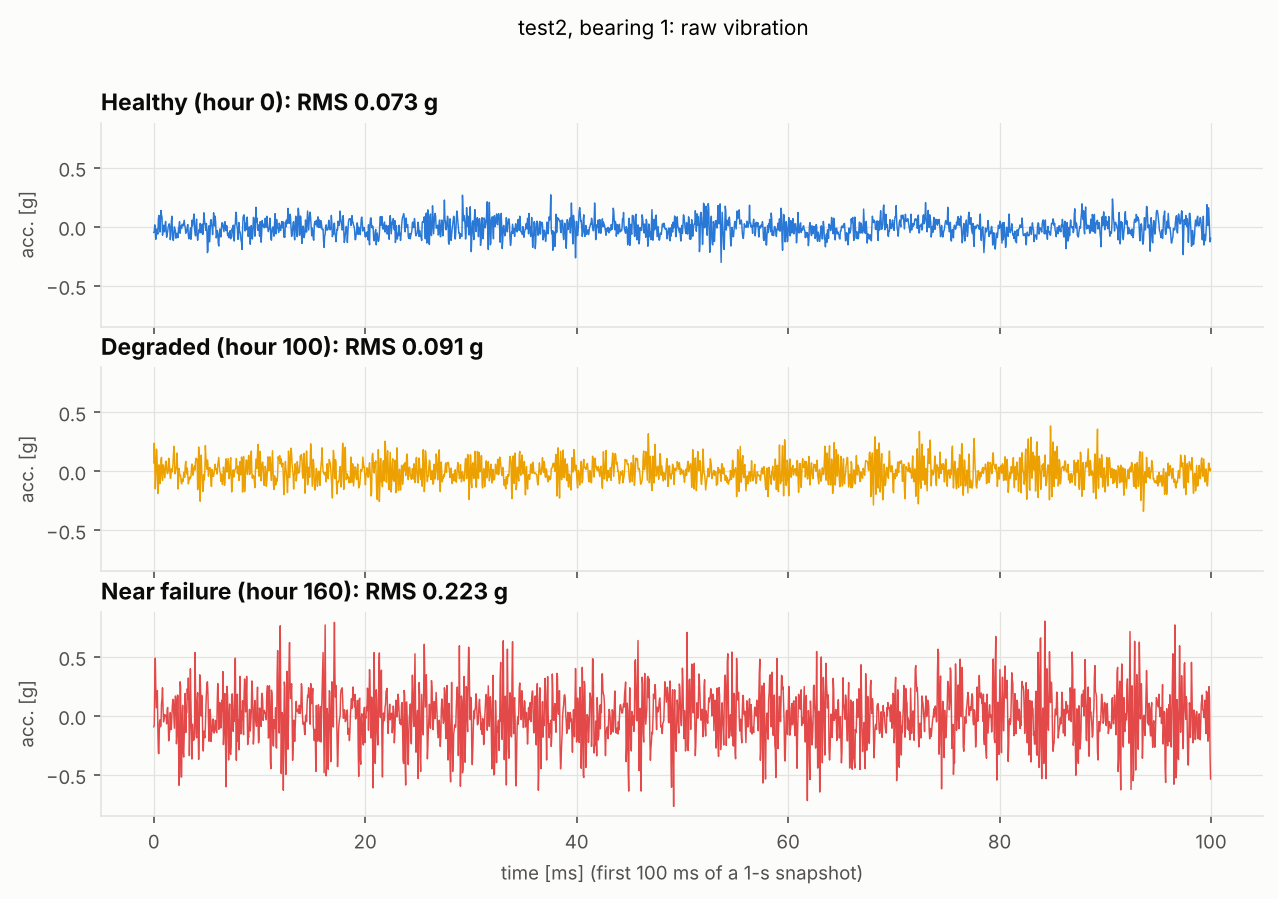
\includegraphics[width=0.92\figw]{report_waveforms.png}
\caption{Raw vibration of test~2, bearing~1 (first 100\,ms of three snapshots).}
\label{fig:wave}
\end{figure}

\textbf{Interpretation.} At hour 100 the waveform is still visually similar to the healthy one and RMS
has risen only from 0.073 to 0.091\,g (+25\,\%), an amount that would be easy to miss by eye or with a
fixed vibration limit. Near failure the amplitude has tripled (0.223\,g) and the signal is clearly
impulsive. An early warning must therefore rely on more than visual inspection of the waveform or the
overall level.

\begin{figure}[H]
\centering
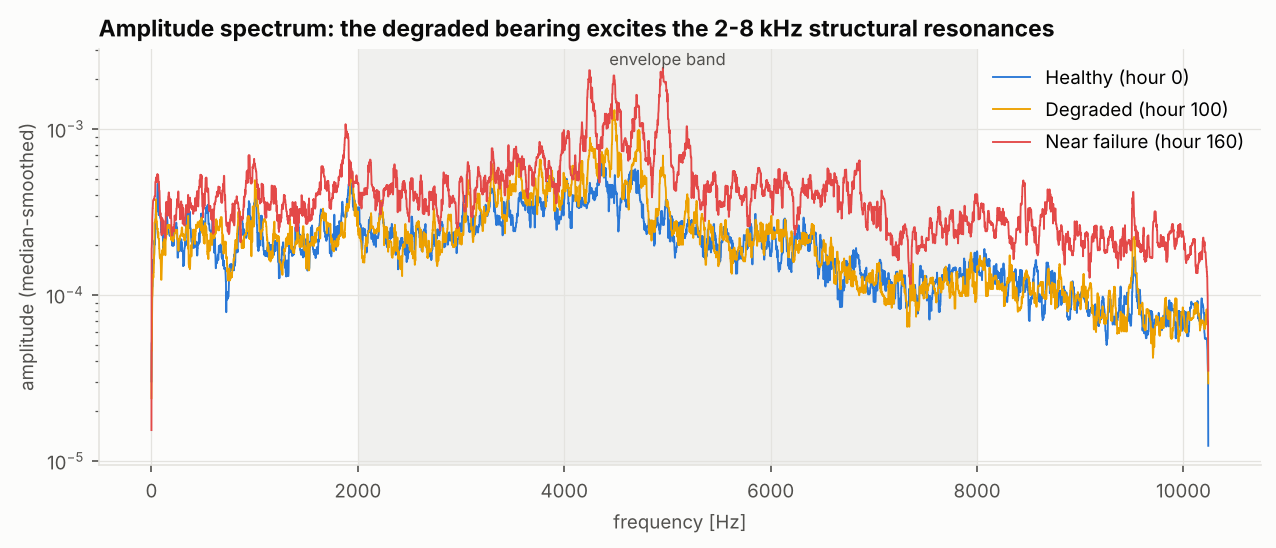
\includegraphics[width=0.92\figw]{report_spectrum.png}
\caption{Amplitude spectrum of the same three snapshots (median-smoothed, log scale).}
\label{fig:spec}
\end{figure}

\textbf{Interpretation.} The energy of all three spectra is concentrated between roughly 3 and 6\,kHz:
these are the structural resonances of the bearing housing. As the bearing degrades, the resonance
peaks grow and broaden, and near failure the high-frequency floor (6--10\,kHz) rises by almost an
order of magnitude. This justifies both the relative band-energy features and the choice of the
2--8\,kHz band for envelope analysis. The spectrum does not, however, show \emph{which} component is
damaged.

\begin{figure}[H]
\centering
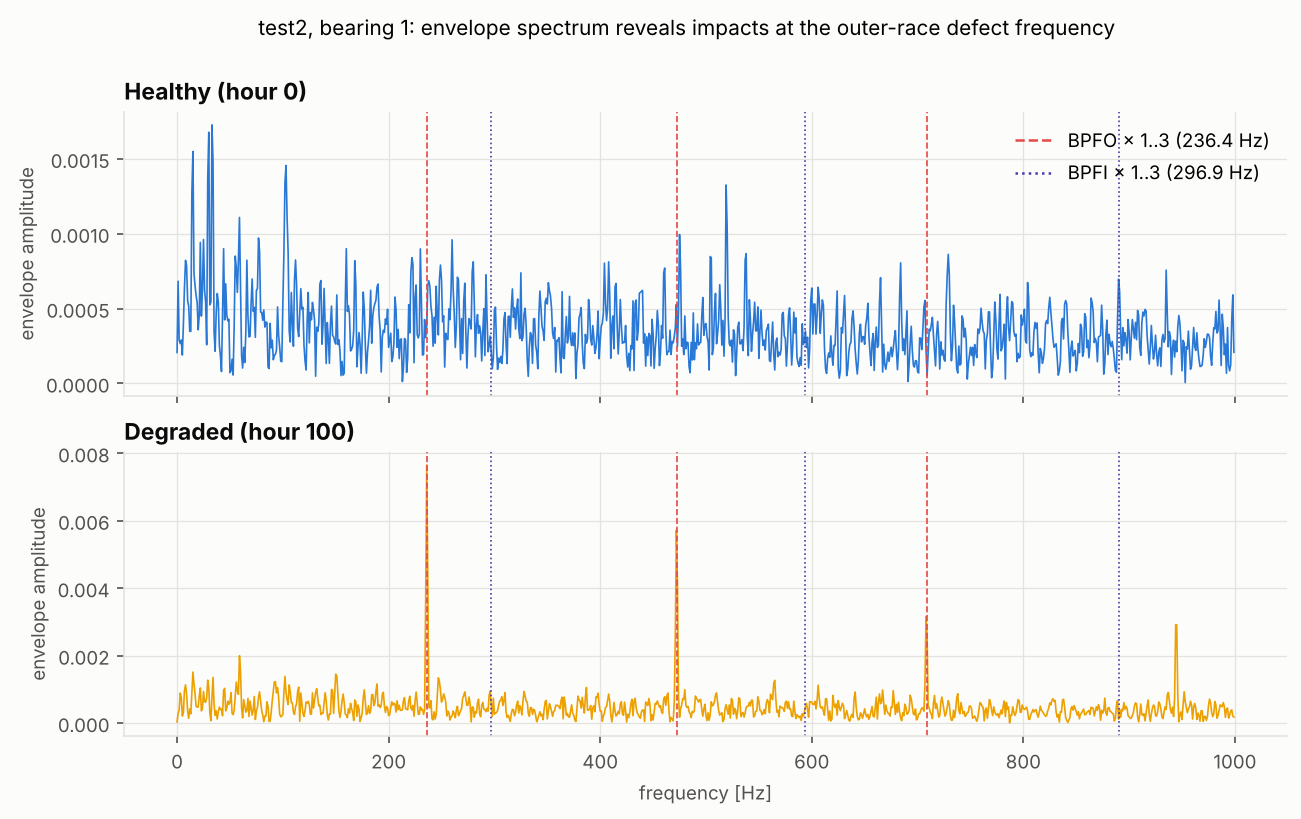
\includegraphics[width=0.92\figw]{report_envelope.png}
\caption{Envelope spectrum of the healthy and degraded snapshots, with the first three harmonics of
BPFO (dashed) and BPFI (dotted).}
\label{fig:env}
\end{figure}

\textbf{Interpretation.} This is the key diagnostic figure. The healthy envelope spectrum is a flat
noise floor with no structure at the defect frequencies. At hour 100 sharp peaks appear exactly at
236, 473 and 709\,Hz, i.e.\ at $1\times$, $2\times$ and $3\times$ BPFO, with amplitudes about ten
times the noise floor, while nothing appears at the inner-race frequencies. This is the textbook
signature of a localized \textbf{outer-race} defect, and it is visible about three days before the end
of the test. It confirms that the bearing geometry, the defect-frequency calculation and the
envelope pipeline are correct, and it is what the \code{env\_bpfo} feature measures.

\subsection{Preprocessing and data splits}
\label{sec:prep}
Features are pivoted into one matrix per bearing (one row per snapshot, ordered in time). Strictly
positive, heavy-tailed features are log-transformed, then every feature is standardized with the mean
and standard deviation of that bearing's own training period (Listing~\ref{lst:prep}). After this step
a value of $+3$ means ``three healthy standard deviations above this bearing's normal'', regardless of
whether the bearing is naturally loud or quiet, so one detector can serve all bearings of a test.

\begin{lstlisting}[caption={Time-ordered splits and per-bearing standardisation (excerpt of \code{src/bearing\_efw/preprocess.py}).},label=lst:prep]
for bearing, w in wide_by_bearing(df).items():
    hours = ((w.index - t0).total_seconds() / 3600).to_numpy()
    # Splits use the snapshot index, not wall-clock time: test1 was recorded in
    # bursts with multi-day gaps, so a time-based split would leave almost no
    # training data.
    life = np.arange(len(w)) / len(w)
    train = life < train_end                       # first 25 %
    calib = (life >= train_end) & (life < calib_end)  # next 10 %

    Z = w.copy()
    log_cols = [c for c in Z.columns if c.rsplit("_ch", 1)[0] in LOG_FEATURES]
    Z[log_cols] = np.log(Z[log_cols].clip(lower=1e-9))
    mu, sd = Z[train].mean(), Z[train].std().replace(0, 1)
    X = ((Z - mu) / sd).to_numpy(dtype=np.float32)
\end{lstlisting}

\begin{table}[H]
\centering
\caption{Size of the splits per bearing.}
\label{tab:splits}
\begin{tabular}{lrrrrr}
\toprule
Test & Snapshots & Train & Calibration & Train ends [h] & Calibration ends [h] \\
\midrule
test1 & 2\,156 & 539   & 216 & 290.1 & 433.8 \\
test2 & 982    & 246   & 98  & 40.8  & 57.2 \\
test3 & 6\,323 & 1\,581 & 633 & 267.5 & 380.2 \\
\bottomrule
\end{tabular}
\end{table}

\subsection{Detectors}
All detectors share one interface: \code{fit} receives the list of healthy training matrices of the
four bearings, and \code{score} maps a bearing's full matrix to one score per snapshot. Fitting on the
pooled, standardized healthy data of all bearings quadruples the training set compared with fitting
one model per bearing.

\begin{lstlisting}[caption={Classical detectors (excerpt of \code{src/bearing\_efw/models.py}).},label=lst:models]
class RMSThreshold:
    """Classic condition-monitoring baseline: overall vibration level (z-score of log RMS)."""
    def fit(self, Xs): return self
    def score(self, X): return X[:, self.idx].max(axis=1)   # idx = RMS columns

class Mahalanobis:
    """Distance from the healthy feature distribution (shrinkage covariance)."""
    def fit(self, Xs):
        self.cov = LedoitWolf().fit(np.vstack(Xs))
        return self
    def score(self, X):
        return np.sqrt(self.cov.mahalanobis(X))

class IForest:
    def __init__(self, n_estimators=300, seed=0):
        self.model = IsolationForest(n_estimators=n_estimators, random_state=seed)
    def fit(self, Xs):
        self.model.fit(np.vstack(Xs))
        return self
    def score(self, X):
        return -self.model.score_samples(X)   # higher = more anomalous
\end{lstlisting}

\paragraph{LSTM autoencoder architecture.} The encoder LSTM (32 hidden units) reads a window of
$W=12$ consecutive snapshots (about two hours); its last hidden state is projected to an 8-dimensional
latent code. The decoder repeats the code over 12 steps, passes it through a second LSTM (32 units)
and a linear layer back to the feature dimension. The model has 16\,250 parameters for 18 features
(19\,148 for test~1's 36 features). It is trained for 60 epochs with Adam (learning rate
$2\times10^{-3}$, batch size 64) as a \emph{denoising} autoencoder: Gaussian noise with standard
deviation 0.1 is added to the input, and the model must reconstruct the clean window. On a training
set of only about 1\,000 windows (test~2) this prevents the network from memorizing the training data.
Windows are built per bearing, never across two bearings, and the window for snapshot $t$ ends at $t$,
so the score only uses past data and can run online.

\begin{lstlisting}[caption={LSTM autoencoder (excerpt of \code{src/bearing\_efw/models.py}).},label=lst:lstm]
class Net(nn.Module):
    def __init__(self):
        super().__init__()
        self.enc = nn.LSTM(n_features, hidden, batch_first=True)
        self.to_latent = nn.Linear(hidden, latent)
        self.from_latent = nn.Linear(latent, hidden)
        self.dec = nn.LSTM(hidden, hidden, batch_first=True)
        self.out = nn.Linear(hidden, n_features)

    def forward(self, x):                       # x: (batch, window, features)
        _, (h, _) = self.enc(x)
        z = self.to_latent(h[-1])               # latent code
        rep = self.from_latent(z).unsqueeze(1).repeat(1, x.shape[1], 1)
        y, _ = self.dec(rep)
        return self.out(y)

def fit(self, Xs):
    # Windows are built per bearing so a sequence never spans two bearings.
    W = torch.tensor(np.concatenate([self._windows(X)[self.window - 1:] for X in Xs]))
    opt = torch.optim.Adam(self.net.parameters(), lr=self.lr)
    for _ in range(self.epochs):
        for idx in np.array_split(self.rng.permutation(len(W)), max(1, len(W) // self.batch_size)):
            xb = W[idx]
            # denoising objective: reconstruct the clean window from a noisy copy
            loss = ((self.net(xb + self.noise * torch.randn_like(xb)) - xb) ** 2).mean()
            opt.zero_grad(); loss.backward(); opt.step()

def score(self, X):
    with torch.no_grad():
        W = torch.tensor(self._windows(X))       # window ending at each snapshot
        return ((self.net(W) - W) ** 2).mean(dim=(1, 2)).numpy()
\end{lstlisting}

\subsection{From scores to alarms}
\paragraph{Threshold.} For each bearing and detector, the threshold is derived from the calibration
scores $s$ only:
\begin{equation}
\tau = Q_{0.995}(s) + m\,\bigl(Q_{0.995}(s) - \operatorname{median}(s)\bigr), \qquad m = 0.5.
\end{equation}
The margin is expressed relative to the spread of the healthy scores, so the rule works for any score
scale and sign (the RMS z-score can be negative, the other scores cannot).

\paragraph{Debouncing.} A single noisy snapshot above $\tau$ should not page an operator. An alarm is
active at snapshot $t$ when at least $k=4$ of the last $n=6$ snapshots (one hour) exceed $\tau$.

\paragraph{Persistent alarm.} A real degradation does not heal. The warning reported for a failed
bearing is the start of the \emph{last} alarm episode, provided it lasts until the end of the record;
earlier episodes that cleared are counted separately.

\begin{lstlisting}[caption={Threshold, k-of-n debouncing and persistent alarm (\code{src/bearing\_efw/alarm.py}).},label=lst:alarm]
def fit_threshold(calib_scores, quantile, margin):
    q, med = np.quantile(calib_scores, quantile), np.median(calib_scores)
    return float(q + margin * (q - med))

def k_of_n(exceed: np.ndarray, k: int, n: int) -> np.ndarray:
    """Alarm at t when at least k of the last n snapshots (inclusive) exceed the threshold."""
    c = np.convolve(exceed.astype(int), np.ones(n, dtype=int))[: len(exceed)]
    return c >= k

def first_persistent_alarm(alarm, hours, start_h):
    """Start of the final alarm episode, if it lasts until the end of the record."""
    eps = [(s, e) for s, e in alarm_episodes(alarm) if hours[s] >= start_h]
    if not eps:
        return None
    return float(hours[eps[-1][0]]) if eps[-1][1] == len(alarm) else None
\end{lstlisting}

\subsection{Diagnosis}
When a persistent alarm is raised, the system looks at the standardized envelope features of the
alarming bearing over the next 12 snapshots and reports the defect frequency with the largest average
z-score, if it exceeds 3 (Listing~\ref{lst:diag}). Otherwise it reports ``no clear defect frequency''
rather than guessing.

\begin{lstlisting}[caption={Envelope-based diagnosis (excerpt of \code{scripts/run\_experiment.py}).},label=lst:diag]
DEFECTS = {"env_bpfo": "outer race", "env_bpfi": "inner race", "env_bsf": "rolling element"}

def diagnose(d, alarm_h, n=12):
    if alarm_h is None:
        return ""
    cols = list(d.raw.columns)
    after = np.flatnonzero(d.hours >= alarm_h)[:n]
    z = {k: np.mean([d.X[after, cols.index(c)].mean() for c in cols if c.startswith(k + "_")])
         for k in DEFECTS}
    best = max(z, key=z.get)
    return f"{DEFECTS[best]} (z={z[best]:.1f})" if z[best] > 3 else "no clear defect frequency"
\end{lstlisting}

\subsection{Evaluation protocol}
The dataset only states that a bearing had failed when each test was stopped; the onset of degradation
is not labelled. Two metrics follow from this:
\begin{itemize}
  \item \textbf{Lead time} of a failed bearing: hours between its persistent alarm and the end of the
        test (also reported as a percentage of the test duration). Higher is better.
  \item \textbf{False alarms}: alarm episodes on \emph{any} bearing inside a window that is believed to
        be healthy: after calibration (35\,\% of snapshots) and before 60\,\%, 50\,\% and 85\,\% of the
        snapshots in tests 1, 2 and 3 respectively. These limits come from inspecting the condition
        indicators (Section~\ref{sec:results}) and are documented in the configuration file. The rate
        is normalised per 1\,000 bearing-hours of that window.
\end{itemize}
Hyper-parameters (split fractions, threshold quantile and margin, $k$ and $n$, network size,
epochs, noise) were chosen on test~2 only. Tests~1 and~3 were not used for any decision and act as
held-out evaluations.

\subsection{Design decisions}
\label{sec:design}
\begin{itemize}
  \item \textbf{Train on the beginning, test on the rest.} All splits are in time order. Shuffling
        windows from the whole run leaks the failure into training.
  \item \textbf{One snapshot is one point in time.} Features are computed per file, so results are in
        hours before failure.
  \item \textbf{Monitor the right bearing, and every bearing.} Each bearing is scored separately; the
        failed bearings are known from the dataset documentation and are only used for evaluation.
  \item \textbf{Split by snapshot count, not wall-clock time.} With test~1's multi-day gaps, the first
        25\,\% of the \emph{time} would contain very few snapshots.
  \item \textbf{Per-bearing baselines.} Standardising each bearing against itself makes one model
        serve bearings with different natural vibration levels.
  \item \textbf{Same threshold rule and alarm logic for all detectors}, so differences in the results
        come from the detectors and not from tuning.
  \item \textbf{Determinism.} All random components are seeded; two consecutive runs produce identical
        result tables.
\end{itemize}

%=====================================================================
\section{Results}
\label{sec:results}
%=====================================================================

\subsection{Headline results}

\begin{table}[H]
\centering
\caption{Lead time of the persistent alarm on each failed bearing (hours before end of test) and false
alarms. Bold: best value per column.}
\label{tab:results}
\small\setlength{\tabcolsep}{4.5pt}
\begin{tabular}{lrrrrr}
\toprule
 & \multicolumn{2}{c}{test1 (held out)} & test2 (dev) & test3 (held out) & False alarms \\
\cmidrule(lr){2-3}
Detector & B3 inner & B4 roller & B1 outer & B3 outer & per 1000 bearing-h \\
\midrule
RMS threshold     & \textbf{99.0} & \textbf{176.6} & 74.3 & \textbf{59.3} & 5.34 \\
Mahalanobis       & 12.2 & 48.0  & 74.3 & 58.7 & 0.67 \\
Isolation Forest  & 12.9 & 156.6 & 72.8 & 14.0 & \textbf{0.00} \\
LSTM autoencoder  & 84.9 & 156.6 & \textbf{74.7} & 58.3 & 12.67 \\
\bottomrule
\end{tabular}
\end{table}

\begin{table}[H]
\centering
\caption{False-alarm episodes per test and size of the evaluation window.}
\label{tab:fa}
\begin{tabular}{lrrr}
\toprule
Detector & test1 & test2 & test3 \\
\midrule
RMS threshold    & 15 & 0 & 1 \\
Mahalanobis      & 0  & 0 & 2 \\
Isolation Forest & 0  & 0 & 0 \\
LSTM autoencoder & 4  & 2 & 32 \\
\midrule
Healthy window (hours) & 434--632 & 57--82 & 380--908 \\
Healthy window (bearing-hours) & 3\,162 & 389 & 8\,443 \\
\bottomrule
\end{tabular}
\end{table}

\begin{figure}[H]
\centering
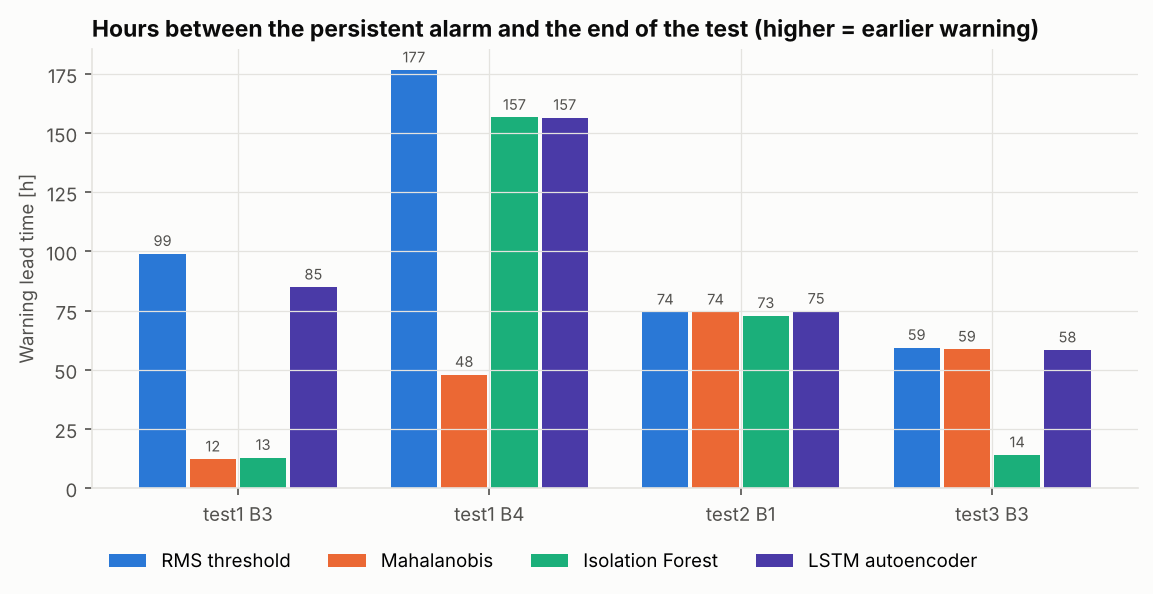
\includegraphics[width=0.95\figw]{lead_times.png}
\caption{Lead time of the persistent alarm for each failed bearing and detector.}
\label{fig:lead}
\end{figure}

\textbf{Interpretation of Figure~\ref{fig:lead}.} On test~2 the four bars are practically equal
(73--75\,h): when a defect develops cleanly, every reasonable detector sees it at the same moment, and
the choice of detector does not matter. The held-out tests separate the detectors. On test~1 the RMS
baseline and the LSTM autoencoder warn earliest (85--177\,h), while Mahalanobis distance warns only
12--48\,h before the end. On test~3 three detectors give about 59\,h and Isolation Forest only 14\,h.
Read together with Table~\ref{tab:fa}, the detectors that warn earliest are also those that raise the
most false alarms; there is no free lunch.

\subsection{Test 2 (development set)}

\begin{figure}[H]
\centering
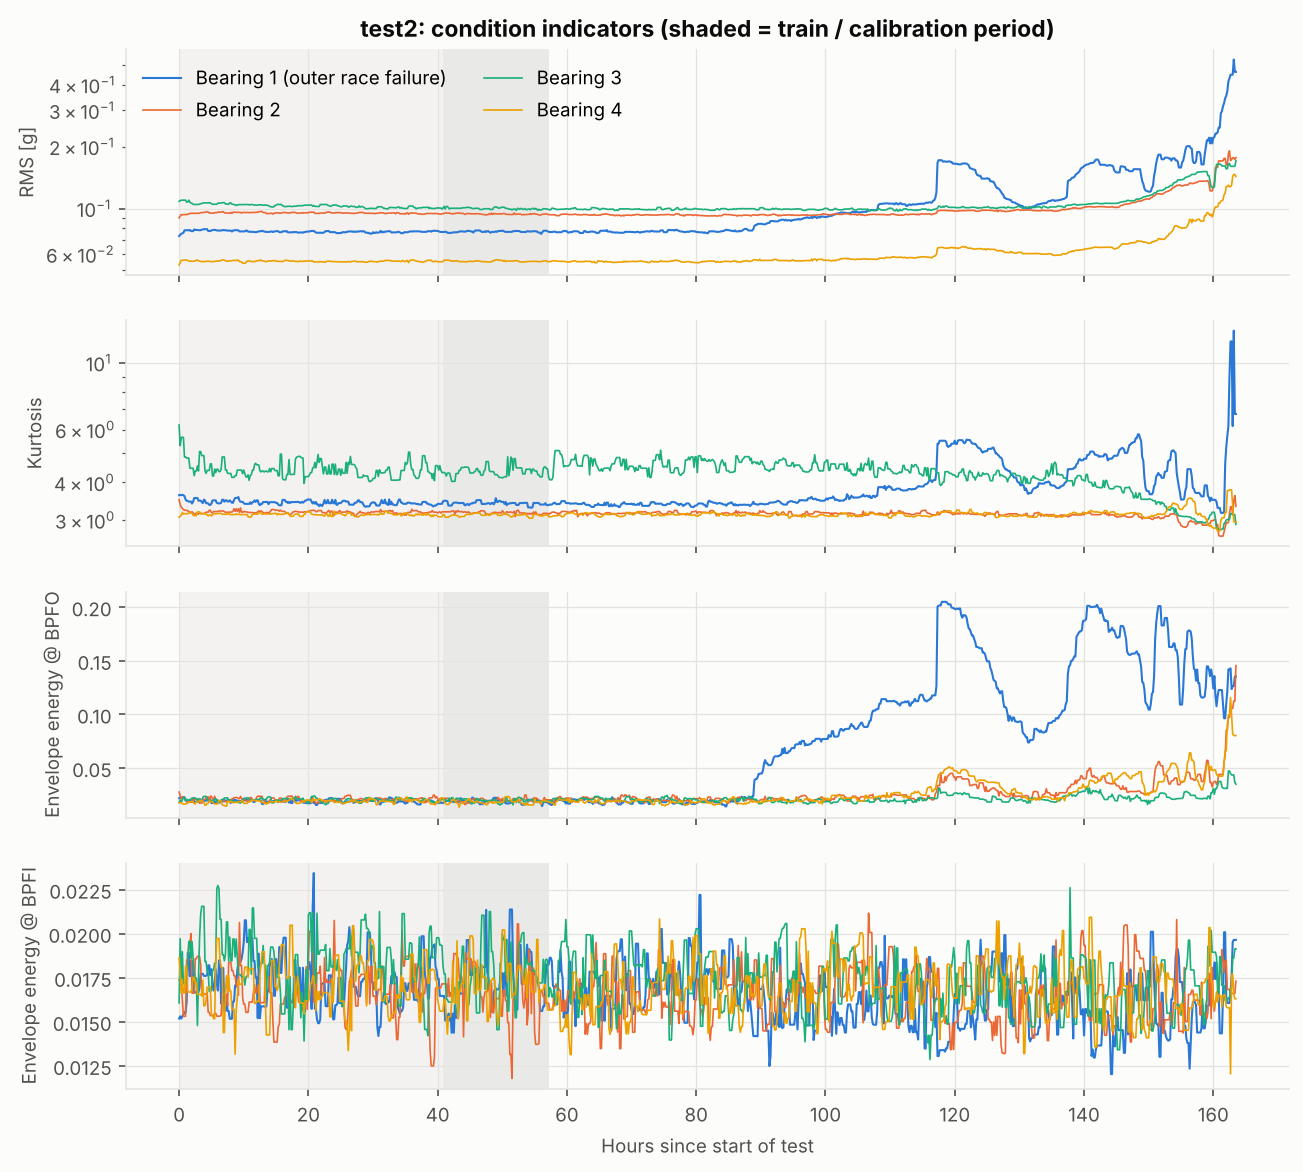
\includegraphics[width=0.93\figw]{test2_indicators.png}
\caption{Condition indicators of test~2 (5-snapshot rolling median). Shaded: training and calibration
periods.}
\label{fig:t2ind}
\end{figure}

\textbf{Interpretation.} For the first 85 hours all four bearings are flat in every indicator.
Around hour 88 the BPFO envelope energy of bearing~1 jumps from 0.02 to 0.05 and keeps rising to
about 0.2 at hour 118, while its RMS increases only slowly; this is the outer-race defect seen in
Figure~\ref{fig:env}. Bearing~1's kurtosis also rises (impacts) but more gradually. The BPFI envelope
energy stays at noise level for all bearings, consistent with an outer-race (not inner-race) defect.
From about hour 115 the other bearings' RMS and BPFO energy also increase: vibration from bearing~1
travels through the shaft and housing. In the last hours all indicators rise steeply. The ``dip'' of
bearing~1's BPFO energy around hour 130 is typical of spall evolution: as the defect edges are worn
smooth the impacts temporarily soften before the damage spreads.

\begin{figure}[H]
\centering
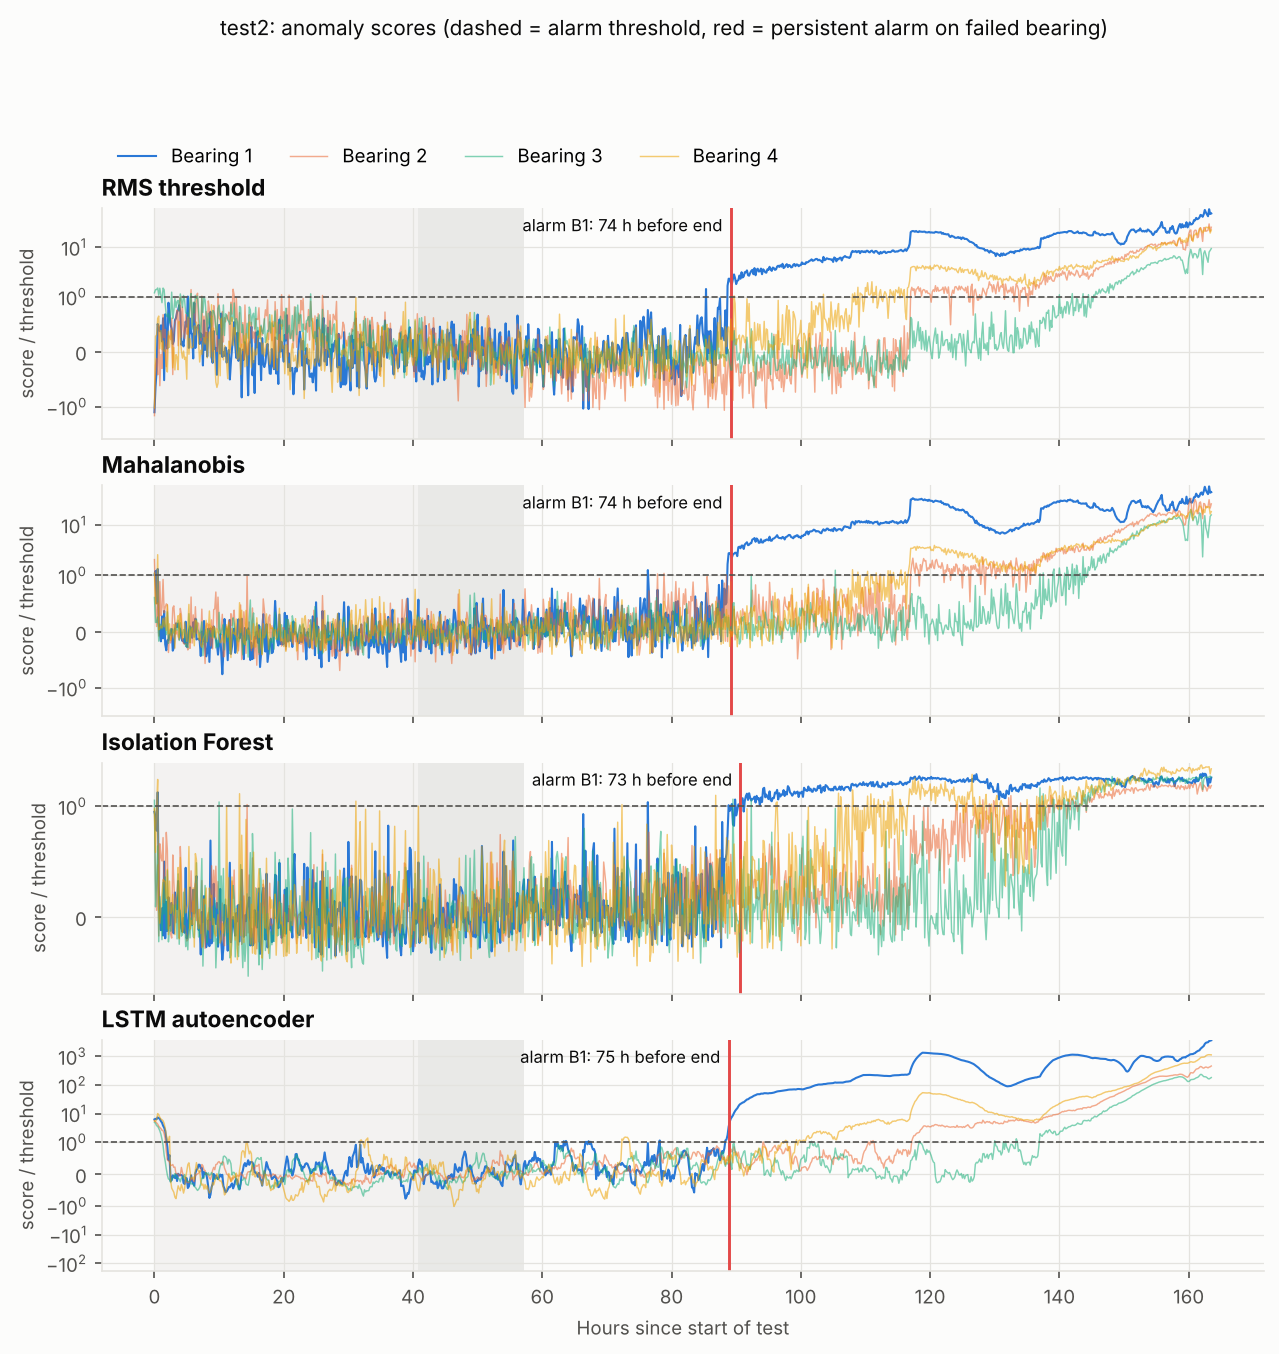
\includegraphics[width=0.93\figw]{test2_detectors.png}
\caption{Test~2 anomaly scores divided by each bearing's threshold (symmetric log scale). Dashed: alarm
threshold; red line: persistent alarm on the failed bearing.}
\label{fig:t2det}
\end{figure}

\textbf{Interpretation.} All four detectors keep every bearing below the threshold during training,
calibration and the following 30 hours, then bearing~1 crosses the threshold at hour 89 and never
returns: a persistent alarm 74\,h before the end. The score jump is largest for the LSTM autoencoder
(two orders of magnitude) and the Mahalanobis distance (about $20\times$), which combine all features,
and smallest for Isolation Forest, whose score saturates by construction. Apart from two short LSTM episodes (which count as false alarms), the
other bearings cross the threshold only after hour 109--145, always after bearing~1, so the
\emph{first bearing to alarm} correctly localises the source. All detectors diagnose an \textbf{outer race} defect at the alarm
(z-scores 6.1--7.3), which is the documented failure mode. Bearings 2 and 4 receive an outer-race
diagnosis too at later alarms, because they pick up bearing~1's vibration; this is why the dashboard
marks the first bearing to alarm as the likely source.

\subsection{Test 1 (held out)}

\begin{figure}[H]
\centering
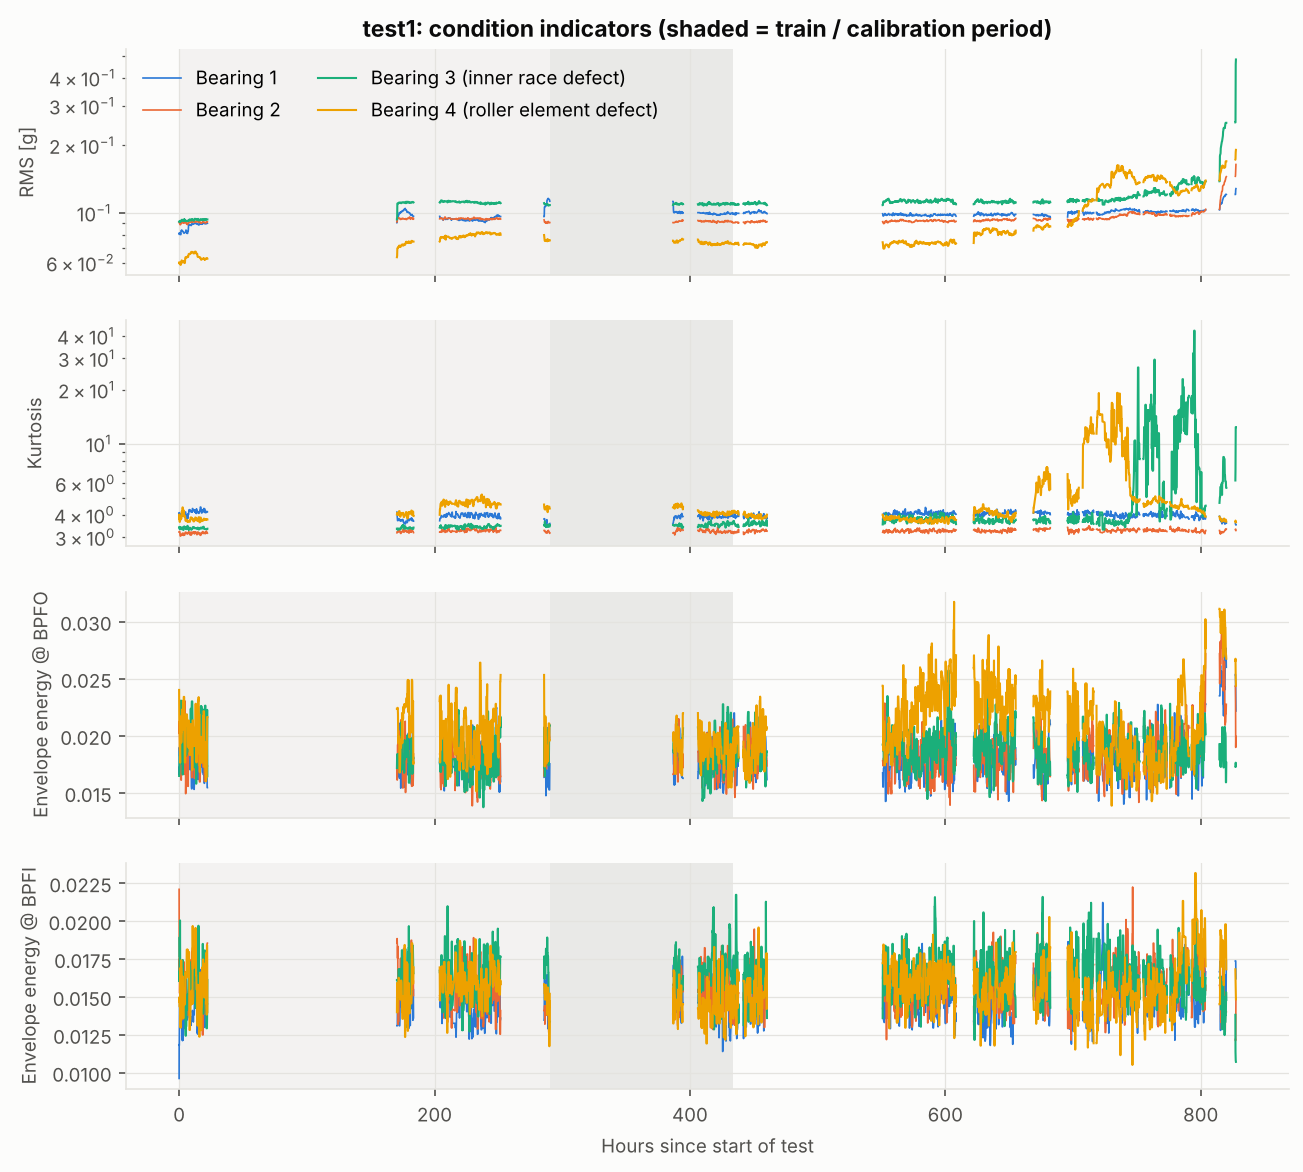
\includegraphics[width=0.93\figw]{test1_indicators.png}
\caption{Condition indicators of test~1. Line breaks are recording gaps.}
\label{fig:t1ind}
\end{figure}

\textbf{Interpretation.} Test~1 is the most difficult record: it is fragmented by gaps of up to six
days, and its training period (the first 539 snapshots, up to hour 290) contains several step changes
between recording bursts, so ``healthy'' is not a single stable state. The degradation of the two
failed bearings is clearly visible in kurtosis: bearing~4 becomes impulsive from about hour 680
(kurtosis up to 20) and bearing~3 from about hour 720 (up to 40), long before their RMS rises. The
envelope energy at BPFI (bearing~3's inner-race defect) does not rise at all, and BPFO energy of
bearing~4 only fluctuates. Inner-race and rolling-element defects rotate in and out of the load zone,
which spreads their envelope energy over sidebands at $\pm f_r$ and the cage frequency rather than
concentrating it at one line; a $\pm3$\,Hz window around the harmonics misses most of it.

\begin{figure}[H]
\centering
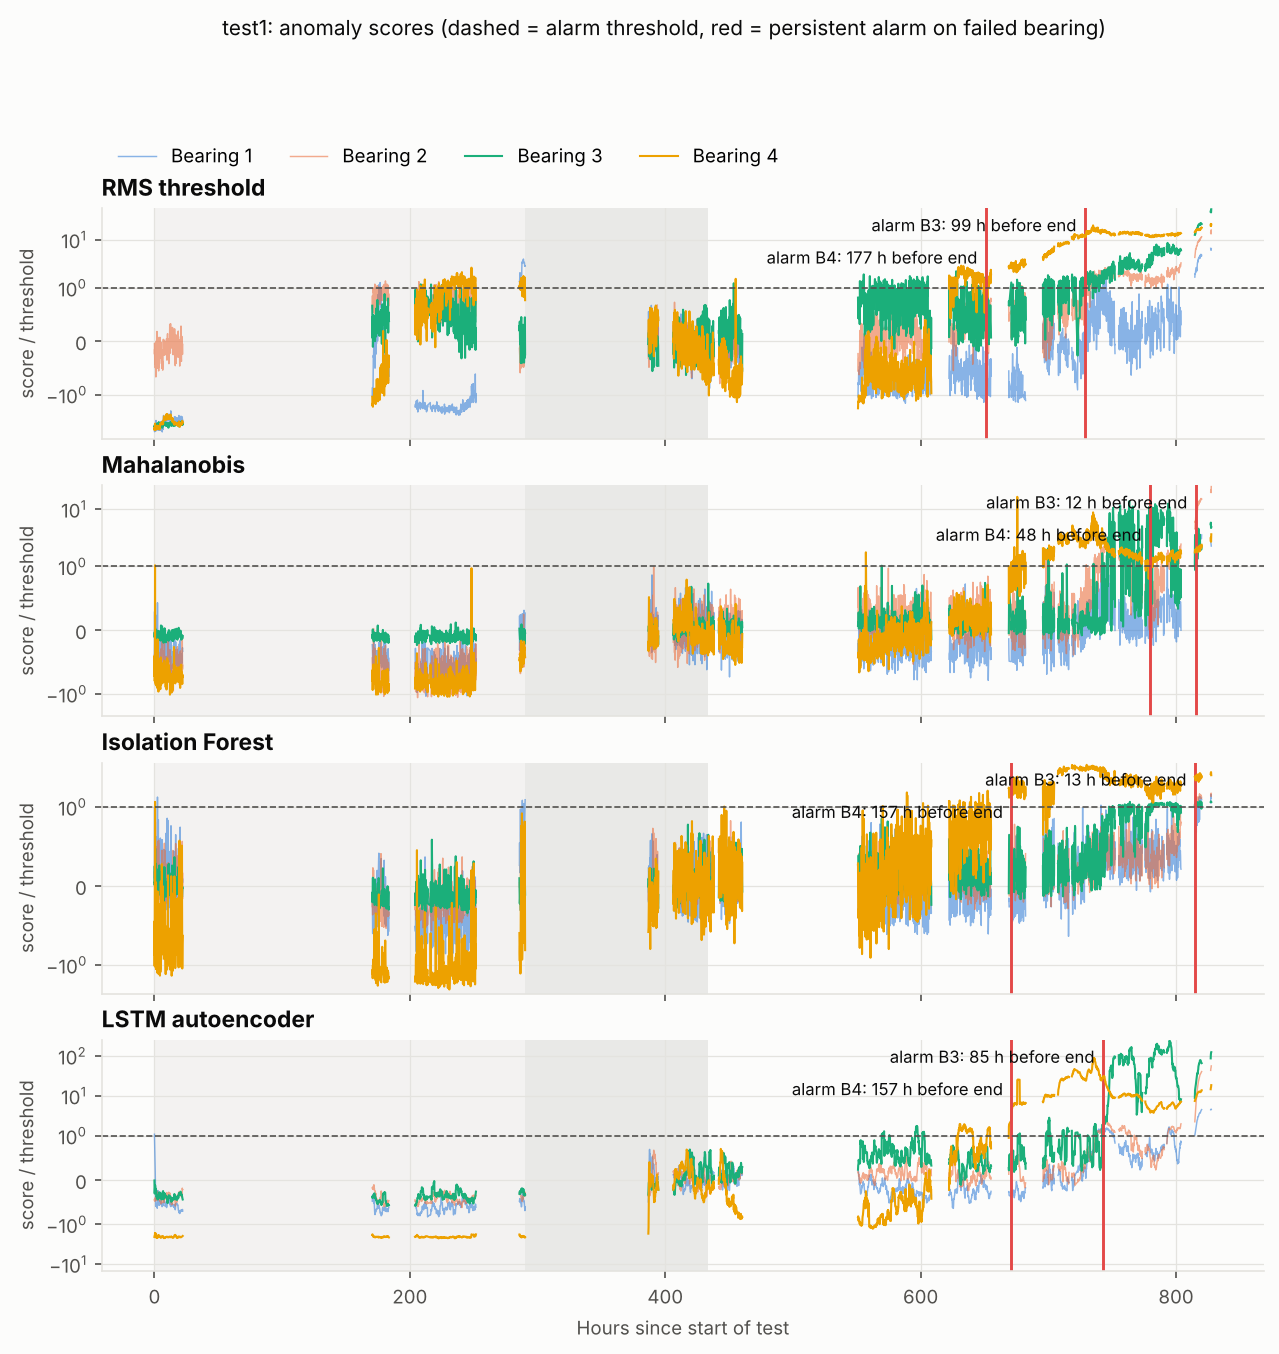
\includegraphics[width=0.93\figw]{test1_detectors.png}
\caption{Test~1 anomaly scores divided by each bearing's threshold.}
\label{fig:t1det}
\end{figure}

\textbf{Interpretation.} Bearing~4 is detected by three detectors 157--177 hours before the end (19--21\,\%
of the run), and both failed bearings are the first to alarm for every detector, so localisation is
correct. The RMS baseline gives the earliest warnings but oscillates around its threshold inside the
assumed-healthy window (hours 434--632), producing 15 alarm episodes on bearings~3 (from hour 554) and~4
(from hour 623). Because these are exactly the two bearings that later fail, some of these episodes
may in fact be the first signs of degradation rather than false alarms; with no labelled onset, the
evaluation conservatively counts them as false. Mahalanobis distance and
Isolation Forest raise none, but their persistent alarm on bearing~3 starts only 12--13\,h before the
end: they also crossed the threshold much earlier (bearing~3 first alarms at 747 and 756\,h) but the
score dipped back below it, so the conservative ``persistent'' definition discards those warnings. The
LSTM autoencoder is the best compromise on this test (85\,h and 157\,h, 4 false-alarm episodes). No
detector produces a confident defect diagnosis on test~1, for the reason given above.

\subsection{Test 3 (held out)}

\begin{figure}[H]
\centering
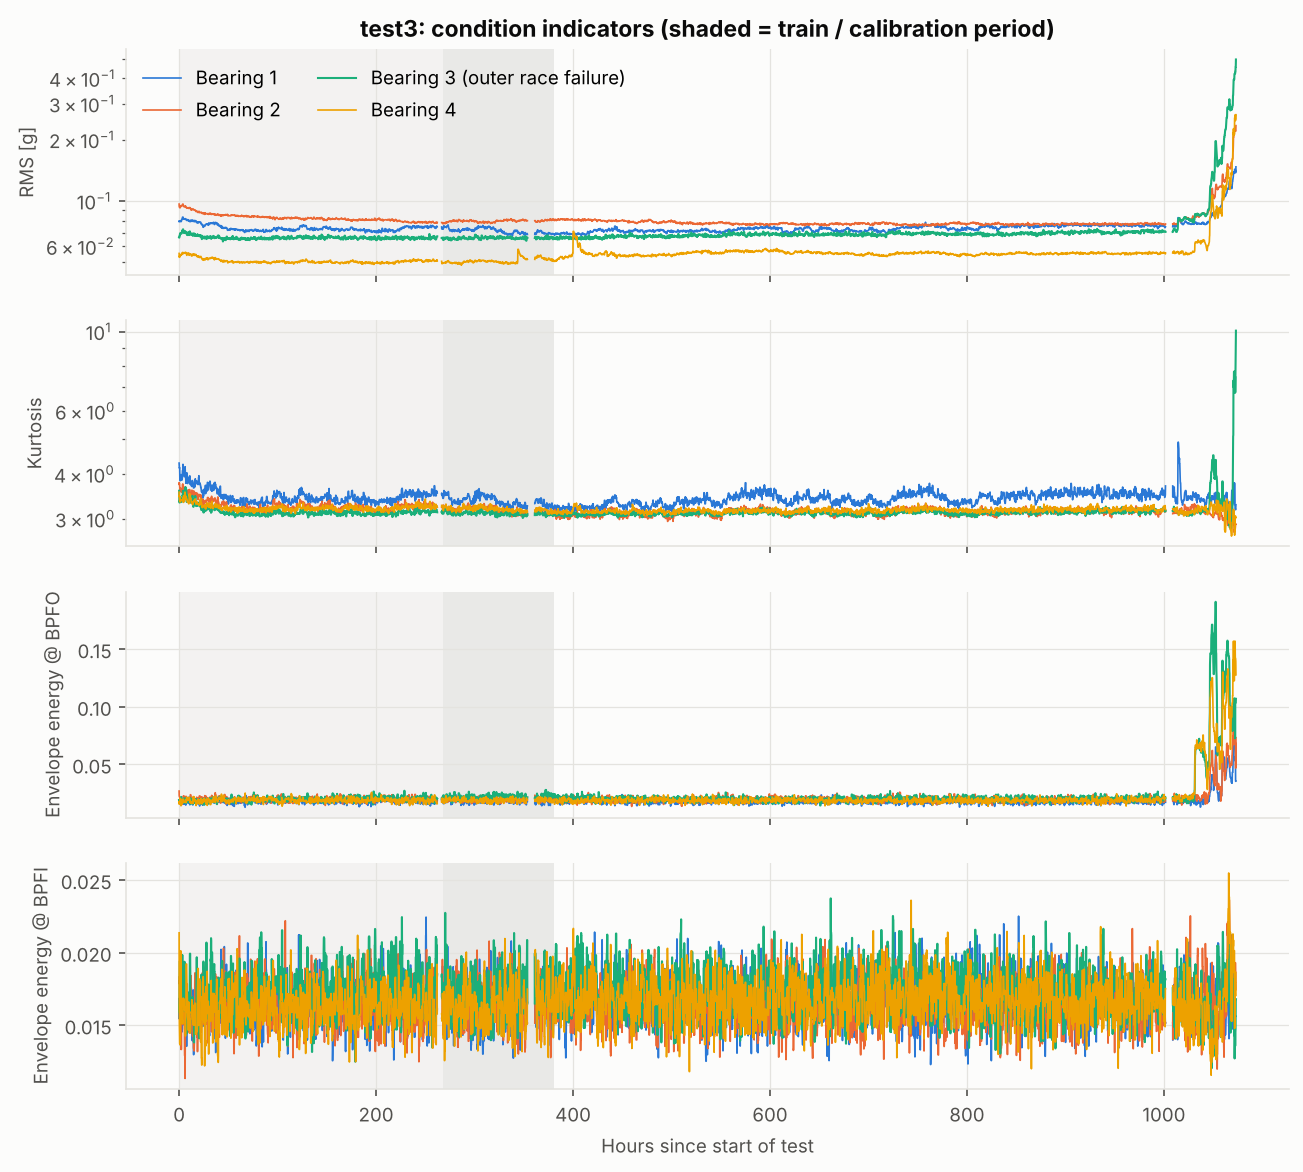
\includegraphics[width=0.93\figw]{test3_indicators.png}
\caption{Condition indicators of test~3.}
\label{fig:t3ind}
\end{figure}

\textbf{Interpretation.} Test~3 shows almost no sign of degradation for 1\,000 hours. Two events
matter. First, after the 7.5-hour stop around hour 354 the RMS of every bearing shifts slightly and
bearing~4 shows a short spike at about hour 400: the machine restarted in a slightly different
condition. Second, after the 7.3-hour stop at hour 1\,002, all indicators change, and from about hour
1\,040 the BPFO envelope energy of bearing~3 (and, through transmission, of bearing~4) rises sharply,
followed by RMS and kurtosis in the last 20 hours. The outer-race defect on bearing~3 therefore
becomes visible only in the last 5\,\% of a 44-day run.

\begin{figure}[H]
\centering
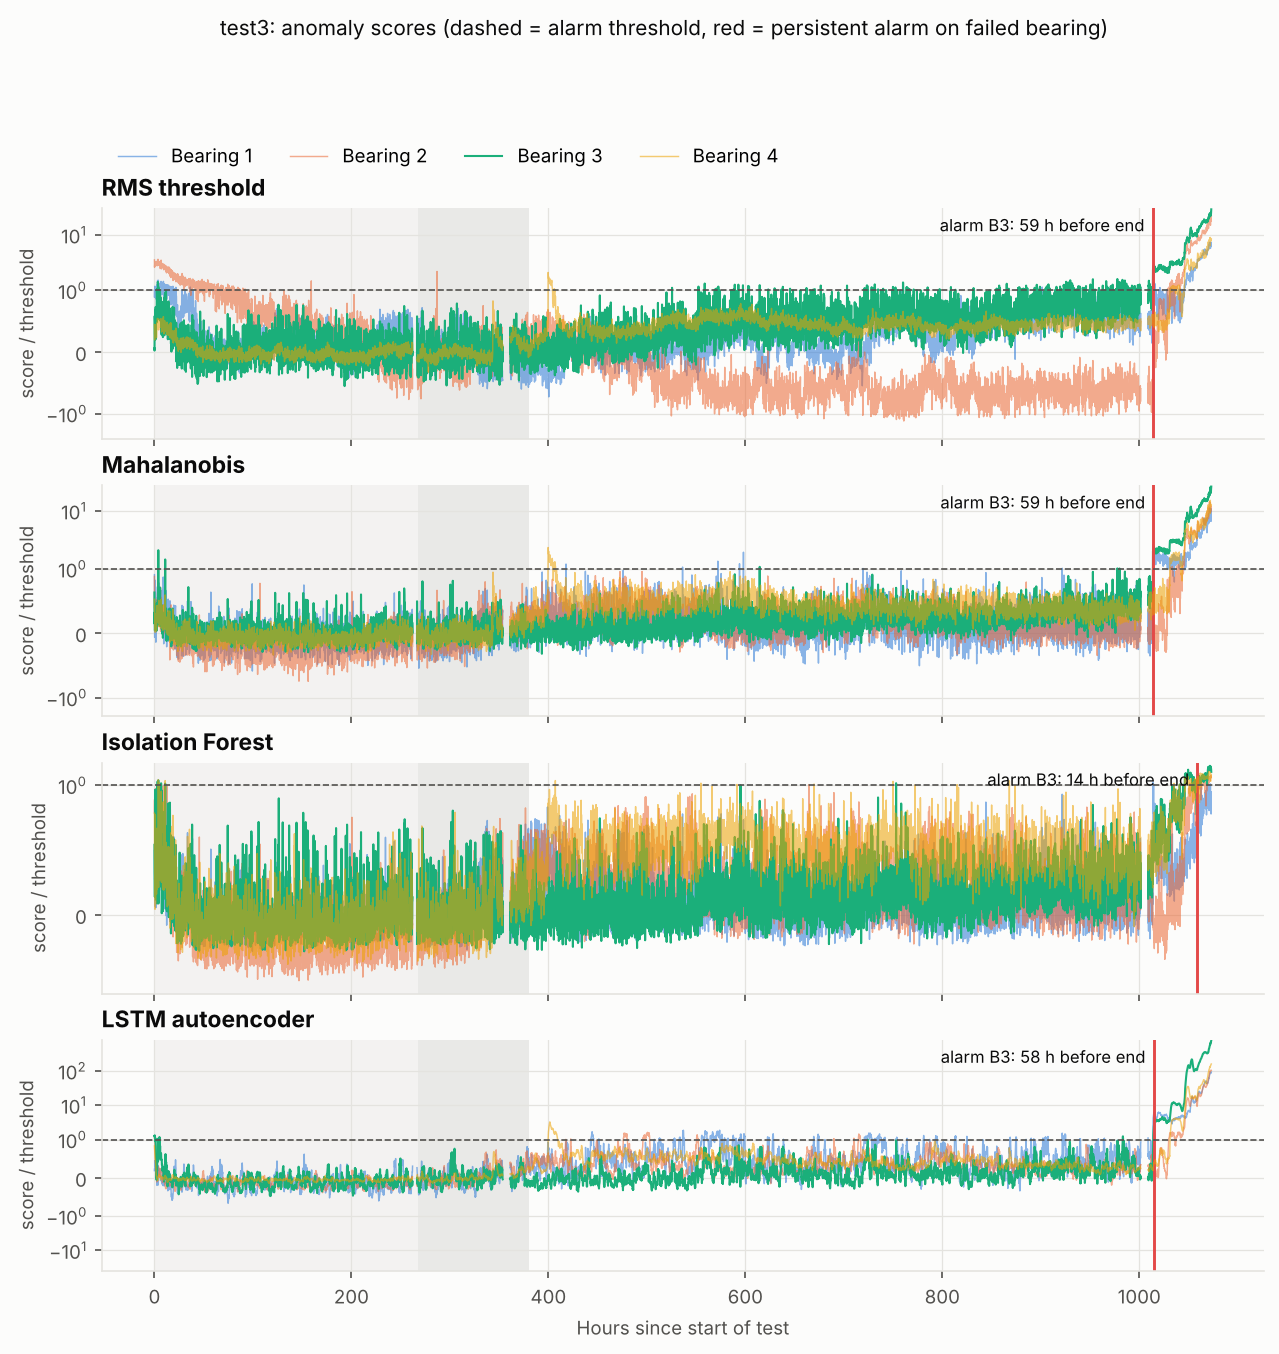
\includegraphics[width=0.93\figw]{test3_detectors.png}
\caption{Test~3 anomaly scores divided by each bearing's threshold.}
\label{fig:t3det}
\end{figure}

\textbf{Interpretation.} The RMS, Mahalanobis and LSTM detectors raise a persistent alarm on bearing~3
about 59\,h before the end, but this alarm starts about 5 hours after recording resumed following the
stop (hour 1\,009) and coincides with alarms on bearing~1. Part of it is therefore a reaction to the restart rather than to the
defect, and these detectors cannot tell which bearing is failing (bearings 1 and 3 alarm within the same
snapshot). Isolation Forest is the only detector whose alarm is unambiguously caused by the defect: it
fires 14\,h before the end, when the BPFO energy surges, and diagnoses an \textbf{outer race} defect with a
z-score of 11.4. The regime shift after hour 354 is the main source of false alarms: the LSTM
autoencoder, which models the joint evolution of all features, interprets the new baseline as anomalous
and raises 32 episodes, mostly on bearing~1. This is the most important limitation of a model trained
once on the beginning of the run.

\subsection{Summary of findings}
\begin{enumerate}
  \item \textbf{Early warning works when the defect develops cleanly.} On test~2 all detectors warn
        74\,h (45\,\% of the run) before the end and name the correct defect.
  \item \textbf{Lead time and false alarms trade off.} The RMS baseline and the LSTM autoencoder warn
        earliest; Isolation Forest never raised a false alarm but warns late on two of four failures;
        Mahalanobis distance sits in between with very few false alarms.
  \item \textbf{A strong baseline matters.} The plain RMS threshold is competitive on lead time. The
        deep model does not dominate on a dataset with only three runs.
  \item \textbf{Localisation by first alarm is reliable} on tests~1 and~2 but not after the restart in
        test~3.
  \item \textbf{Envelope diagnosis is reliable for outer-race defects} (tests~2 and~3) but does not
        recognise test~1's inner-race and roller defects with the current narrow-band feature.
  \item \textbf{Operating-condition changes} (restarts, maintenance) are the main threat to
        validity: a model fitted once on the beginning of life treats a new normal as an anomaly.
\end{enumerate}

%=====================================================================
\section{Interactive dashboard}
%=====================================================================
To show how the system would look to an operator, \code{app/dashboard.py} replays any test as if it
were streaming from the machine (Figure~\ref{fig:dash}). The user selects a test and a detector and
presses \emph{Play}; the dashboard advances snapshot by snapshot and shows:
\begin{itemize}
  \item a status tile per bearing (healthy / above threshold / alarm) with a colour, icon and label,
        the score-to-threshold ratio, the time since the current alarm started, a
        \emph{first to alarm} marker for the likely source, and the diagnosed defect;
  \item the anomaly-score chart of all bearings up to the current time, with the training and
        calibration periods shaded;
  \item the envelope z-scores at BPFO, BPFI and BSF for a selected bearing;
  \item an alarm log and, on request, the ground truth (which bearing failed and how).
\end{itemize}

\begin{figure}[H]
\centering
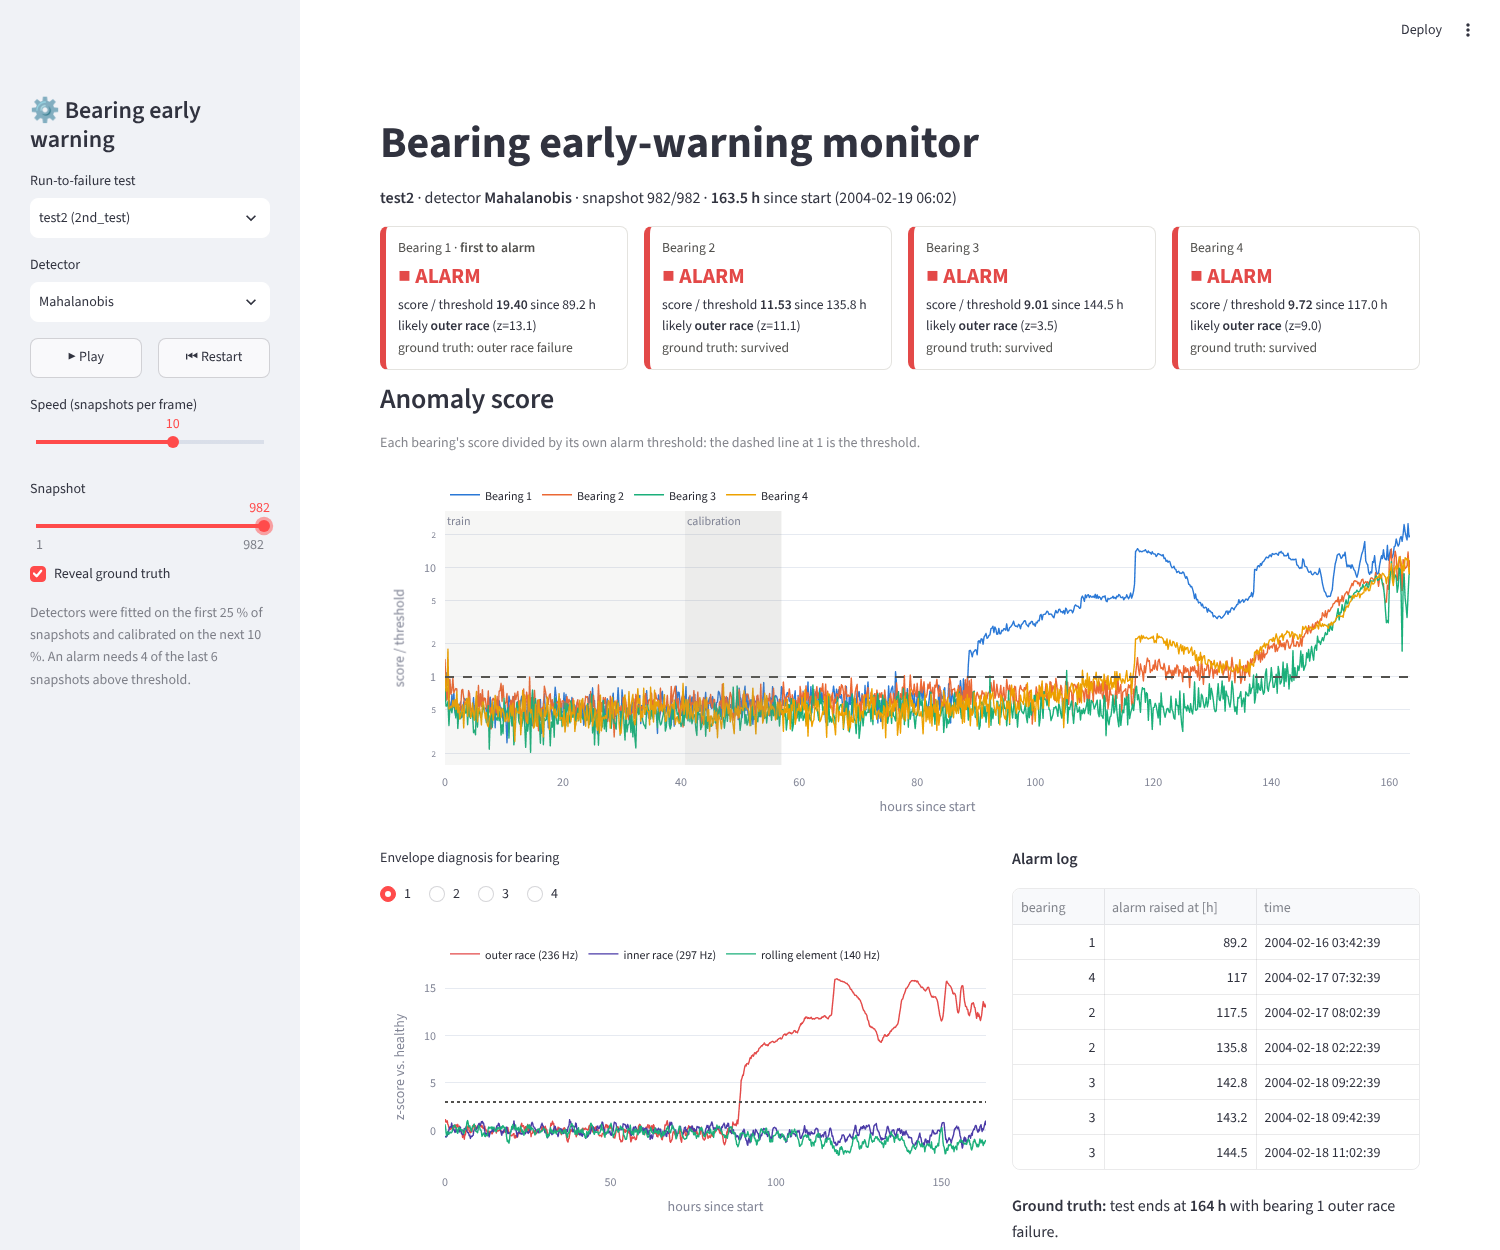
\includegraphics[width=0.95\figw]{dashboard.png}
\caption{Dashboard at the end of test~2 with the Mahalanobis detector and ground truth revealed.}
\label{fig:dash}
\end{figure}

\textbf{Interpretation.} The tiles summarise the story of test~2 in one line: bearing~1 is the first to
alarm (since hour 89.2) with a clear outer-race signature (z = 13.1), the others follow 28--55 hours
later. The envelope chart shows the BPFO z-score of bearing~1 jumping from 0 to above 10 around hour
90 while BPFI and BSF stay flat: the evidence behind the diagnosis is visible to the operator.

\begin{lstlisting}[caption={Likely source and status of each bearing (excerpt of \code{app/dashboard.py}).},label=lst:dash]
# The first bearing to raise an alarm is the likely source: once it degrades, its
# vibration travels through the shaft and housing and lifts its neighbours too.
onsets = {b: g.loc[g["alarm"], "hours"].min() for b, g in seen.groupby("bearing") if g["alarm"].any()}
source = min(onsets, key=onsets.get) if onsets else None

for col, (b, g) in zip(cols, seen.groupby("bearing")):
    last = g.iloc[-1]
    state = "alarm" if last.alarm else ("watch" if last.score > last.threshold else "ok")
    defect, zval = diagnose(zs[b].loc[:now])      # mean z of the last 6 snapshots
    ...

# Playback: advance the slider and rerun the script
if st.session_state.playing and idx < n:
    st.session_state["advance_to"] = min(n, idx + speed)
    time.sleep(0.15)
    st.rerun()
\end{lstlisting}

The dashboard reads only the committed result files, so it runs without the raw dataset:
\code{make dashboard} opens it at \code{http://localhost:8501}.

%=====================================================================
\section{Software engineering and reproducibility}
%=====================================================================

\subsection{Repository layout}
\begin{lstlisting}[style=plain]
configs/default.yaml      splits, thresholds, alarm rule, model hyper-parameters
src/bearing_efw/
    dataset.py            test metadata, bearing geometry, defect frequencies, loader
    features.py           time, spectral and envelope features per snapshot
    preprocess.py         per-bearing matrices, log + standardisation, splits
    models.py             RMS, Mahalanobis, Isolation Forest, LSTM autoencoder
    alarm.py              thresholding, k-of-n debouncing, alarm episodes
    plots.py              report figures
scripts/                  download_data, build_features, run_experiment, make_report_figures
app/dashboard.py          Streamlit replay dashboard
data/features/            extracted features (committed, 3 MB)
reports/                  results.md, summary.csv, scores.csv.gz, figures/
notebooks/                01_walkthrough.ipynb
tests/                    unit tests and dashboard smoke tests
report/                   this report (LaTeX sources and PDFs, English and Turkish)
\end{lstlisting}

\subsection{Configuration}
Every experimental choice lives in one YAML file, so the experiment can be changed without touching
code:
\begin{lstlisting}[style=plain]
split:      {train_end: 0.25, calib_end: 0.35}
healthy_end: {test1: 0.60, test2: 0.50, test3: 0.85}
threshold:  {quantile: 0.995, margin: 0.5}
alarm:      {k: 4, n: 6}
models:
  isolation_forest: {n_estimators: 300, seed: 0}
  lstm_ae: {window: 12, hidden: 32, latent: 8, epochs: 60, lr: 0.002,
            batch_size: 64, noise: 0.1, seed: 0}
\end{lstlisting}

\subsection{Running}
\begin{lstlisting}[style=plain]
pip install -r requirements.txt
make experiment   # ~2 min, uses the committed feature tables
make dashboard    # interactive replay at http://localhost:8501
make test
make data         # optional: download + extract raw data (~1 GB / 6 GB)
make features     # optional: rebuild the feature tables from raw data
\end{lstlisting}

\subsection{Testing}
Twelve automated tests check the parts most likely to break silently. The most important one builds a
synthetic outer-race defect (resonance bursts repeating exactly at BPFO, buried in noise) and checks
that the envelope feature detects it and attributes it to the outer race (Listing~\ref{lst:test}).
Other tests check the defect frequencies against the published values, the statistics of Gaussian
noise (RMS $=1$, kurtosis $=3$), the debouncing and persistence logic, the threshold's invariance to a
score shift, and that the dashboard renders without errors for every test with two detectors.

\begin{lstlisting}[caption={Synthetic fault test (excerpt of \code{tests/test\_core.py}).},label=lst:test]
def test_envelope_picks_up_outer_race_impacts():
    """Synthetic outer-race defect: resonance bursts repeating at BPFO."""
    rng = np.random.default_rng(1)
    t = np.arange(FS) / FS
    bpfo = fault_frequencies()["bpfo"]
    impacts = np.zeros(FS)
    impacts[(np.arange(0, 1, 1 / bpfo) * FS).astype(int)] = 1.0
    ring = np.exp(-t[:200] * 2000) * np.sin(2 * np.pi * 4000 * t[:200])
    faulty = np.convolve(impacts, ring)[:FS] * 3 + 0.3 * rng.standard_normal(FS)
    healthy = 0.3 * rng.standard_normal(FS)
    f_faulty, f_healthy = snapshot_features(faulty), snapshot_features(healthy)
    assert f_faulty["env_bpfo"] > 5 * f_healthy["env_bpfo"]
    assert f_faulty["env_bpfo"] > f_faulty["env_bpfi"]
    assert f_faulty["kurtosis"] > f_healthy["kurtosis"]
\end{lstlisting}

\subsection{Version control}
The project is hosted on GitHub (\url{https://github.com/ecemaydemir/bearing_early_fault_warning}).
The initial pipeline was committed to \code{main}; later additions (the dashboard, this report) were
developed on separate branches and merged through pull requests.

%=====================================================================
\section{Discussion and limitations}
%=====================================================================
\begin{itemize}
  \item \textbf{Ground truth.} Only ``failed at the end of the test'' is known. Lead time therefore
        measures how early an alarm persists, not detection of a known onset, and the healthy windows
        used for false alarms are a documented judgement.
  \item \textbf{Small sample.} Three runs and four failed bearings are not enough for statistically
        robust rankings; numbers will move with other settings. Settings were chosen on test~2 only to
        keep the held-out results honest.
  \item \textbf{Non-stationary operation.} Restarts in test~3 move every bearing's baseline. In a real
        plant, the baseline would be re-estimated after maintenance or when an operator confirms that a
        change is benign.
  \item \textbf{Narrow-band diagnosis.} Inner-race and rolling-element defects are modulated by
        shaft and cage rotation; sideband-aware or spectral-kurtosis-based band selection would make the
        diagnosis more general.
  \item \textbf{Persistence is conservative.} Requiring the alarm to persist until the end removes
        intermittent but real early warnings (test~1, bearing~3); in practice, an intermittent alarm is
        itself useful information for the operator.
\end{itemize}

%=====================================================================
\section{Conclusion and future work}
%=====================================================================
The project delivers a working, reproducible early-warning pipeline for bearings that uses no failure
labels. On the cleanest run it warns three days (45\,\% of the run) ahead and names the right defect;
on the harder runs it makes the trade-off between lead time and false alarms explicit and documents
where and why it fails. The most valuable next steps are:
\begin{enumerate}
  \item adaptive re-baselining after restarts and maintenance (test~3);
  \item remaining-useful-life estimation after the alarm, e.g.\ by fitting a degradation trend to the
        health indicator;
  \item sideband-aware envelope features or spectral kurtosis for inner-race and rolling-element
        diagnosis;
  \item an ensemble alarm (e.g.\ two of four detectors) to combine early warning with few false alarms;
  \item validation on other run-to-failure datasets (e.g.\ FEMTO/PRONOSTIA, XJTU-SY).
\end{enumerate}

\begin{thebibliography}{9}
\bibitem{lee2007} J.~Lee, H.~Qiu, G.~Yu, J.~Lin, and Rexnord Technical Services.
  \emph{Bearing Data Set}. IMS, University of Cincinnati. NASA Prognostics Data Repository, NASA Ames
  Research Center, 2007.
\bibitem{qiu2006} H.~Qiu, J.~Lee, J.~Lin, and G.~Yu. Wavelet filter-based weak signature detection
  method and its application on rolling element bearing prognostics. \emph{Journal of Sound and
  Vibration}, 289(4--5):1066--1090, 2006.
\bibitem{randall2011} R.~B.~Randall and J.~Antoni. Rolling element bearing diagnostics---A tutorial.
  \emph{Mechanical Systems and Signal Processing}, 25(2):485--520, 2011.
\bibitem{liu2008} F.~T.~Liu, K.~M.~Ting, and Z.-H.~Zhou. Isolation forest. In \emph{Proc. IEEE
  International Conference on Data Mining}, pages 413--422, 2008.
\bibitem{ledoit2004} O.~Ledoit and M.~Wolf. A well-conditioned estimator for large-dimensional
  covariance matrices. \emph{Journal of Multivariate Analysis}, 88(2):365--411, 2004.
\bibitem{hochreiter1997} S.~Hochreiter and J.~Schmidhuber. Long short-term memory. \emph{Neural
  Computation}, 9(8):1735--1780, 1997.
\bibitem{malhotra2016} P.~Malhotra et al. LSTM-based encoder-decoder for multi-sensor anomaly
  detection. \emph{ICML Anomaly Detection Workshop}, 2016.
\end{thebibliography}

\end{document}
